\section{Założenia projektowe}
W tym rozdziale opisane zostały problemy na jakie można natknąć się w trakcie jego implementacji, wraz z wyszczególnieniem dostępnych rozwiązań. Następnie scharakteryzowana została wybrana architektura aplikacji i szczegółowo opisano jej schemat wraz z pakietami wykorzystanymi do jego implementacji. Omówiono również środowisko programistyczne w jakim będzie działać emulator.

\subsection{Opis problemu i dostępnych rozwiązań}
Podstawowym problemem przy projektowaniu emulatora jest implementacja modułu procesora. To on odpowiada za obliczenia, przetwarzanie pamięci \textit{RAM} oraz zarządzanie rejestrami. Jego działanie jest ściśle określone poprzez zestaw instrukcji, które nieodpowiednio przetłumaczone na język programowania, zaburzają działanie całego programu, generując przy tym trudne do odnalezienia błędy. W tym przypadku, sprawdza się dobrze zaprojektowana struktura kodu, oparta na zasadach \textit{KISS} (\textit{ang. \textit{Keep It Simple}}) i \textit{DRY} (\textit{Don't Repeat Yourself}), dbających o zachowanie klarowności kodu projektu. Pomagają w tym równie, testy jednostkowe, które poza tym mogą sprawdzać, czy dany fragment programu zachowuje się tak, jak zaplanował to programista. Nie chronią one jednak przed błędami wynikającymi ze nieścisłości w  napisanej specyfikacji technicznej, czy też jej niewłaściwym zrozumieniem. Dlatego, aby dobrze zapoznać się z instrukcjami CHIP-8 warto dopisać moduł zajmujący się deasembleracją kodu bitowego wczytanego z programu działającego na tę platformę, będzie on również pomocny przy ewentualnym odnajdywania błędów emulatora. Inną dobrą praktyką jest implementacja własnego debuggera, który na bierząco wskazywałby na wykonywaną instrukcję, a także wyświetlałby bieżący stan rejestrów.
Emulator musi posiadać moduł odpowiedzialny za wyświetlanie grafiki, dźwięki i obsługę urządzeń wejścia. Istnieje wiele dostępnych pakietów napisanych w języku Python, takich jak Tkinter, PyQT oraz wxWidgets nadających się do implementacji tych funkcji. Dobrym rozwiązaniem jest także wykorzystanie bibliotek odpowiedzialnych za grafikę, takich jak pyglet, bezpośrednio odnoszących się do OpenGL lub skierowanych do tworzenia gier: pygame, arcade.
Istotnym problemem jest również interakcja z użytkownikiem i dostarczenie mu interfejsu do wczytywania \textit{obrazów ROM}.

\subsection{Architektura systemu}
Architektura aplikacji została przemyślana tak, aby każdy z modułów odpowiadał za inną funkcje, oddzielając poszczególne warstwy abstrakcji. Komponent odpowiedzialny za pamięć, przechowuje wczytane dane, które następnie są przetwarzane przez moduł symulujący jednostkę obliczeniową i wyświetlane użytkownikowi w warstwie \textit{wyjścia/wejścia}. Zewnętrzne interakcje są również przekazywane przez warstwę prezentacji do opracowania przez procesor, a przy chęci zmiany wczytanego przez emulator programu, żądanie to trafia do procesora, który następnie usuwa dane trzymane w module pamięci. Koncepcji tej odpowiada \textit{architektura warstwowa} \cite{Richards}.

\begin{figure*}[!htb]
\begin{center}
	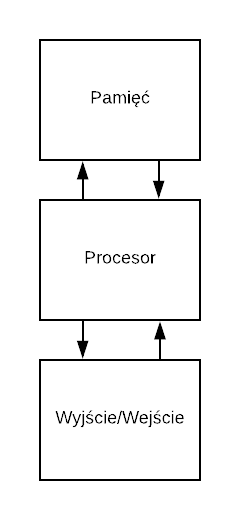
\includegraphics[scale=0.4]{images/architectureDiag}
	\caption{Uproszczony diagram architektury systemu}
\end{center}
\end{figure*}

\newpage

\subsection{Struktura klas}
Struktura klas została oparta na \textit{agregacji}, czyli relacji, która charakteryzuje się, tym, że jeden obiekt jest właścicielem kolejnego, może być on również współdzielony. Klasy \textit{Processor} i \textit{Disassembler} posiadają atrybut o nazwie \textit{memory}, który przechowuje instancje klasy \textit{Memory}. Podobnie jest z strukturą obiektu \textit{Screen}, gdzie pole \textit{proc}, trzyma instancje \textit{Processor}, która dodatkowo jest współdzielona z klasą \textit{Window}. Z kolei relacja między tymi klasami to \textit{kompozycja}. Charakteryzuje się ona tym, że obiekt zagregowany ma taki sam czas życia jak jego właściciel, dodatkowo jego istnienie poza nim nie ma sensu \cite{Trybulec}. \\

Dla uproszczenia na diagramie poniżej nie ma wypisanych metod związanych z obsługą instrukcji procesora, ze względu na ich ilość. Są one oznaczone jedynie jako \textit{instruction functions}. Na schemacie nie ma również graficznego odniesienia do biblioteki \textit{tkinter}. Relacja. dziedziczenia pomiędzy nią, a obiektem \textit{Window} została zasygnalizowana w nawiasach obok nazwy klasy.

\begin{figure*}[!htb]
\begin{center}
	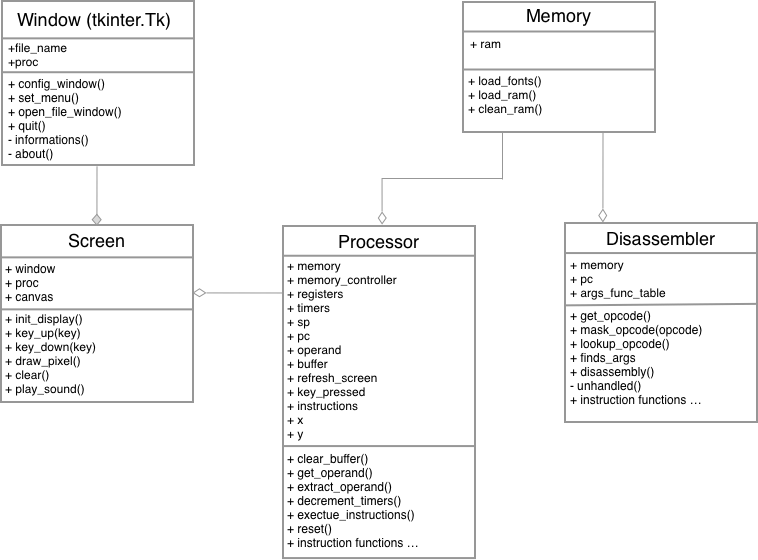
\includegraphics[scale=0.4]{images/class_scheme}
	\caption{Uproszczony diagram schematu klas}
\end{center}
\end{figure*}

\subsection{Wykorzystane biblioteki}
W celu napisania projektu wykorzystano następuje biblioteki:
\begin{itemize}
	\item \textit{Tkinter}, jest to zorientowany obiektowo pakiet napisany jako warstwa dla języka Tcl/Tk \cite{TKINTER}. Dostarcza on niezależne od systemu operacyjnego narzędzia do tworzenia aplikacji okienkowych, włącznie z obsługą multimediów i urządzeń wejścia, takich jak klawiatura, czy mysz komputerowa. Moduł ten od wersji języka Python 3.0 zawiera się \textit{Standardowej Bibliotece Pythona} \footnote{Zestaw pakietów i modułów dostarczanych wraz z instalatorem języka Python, ich wykaz dostępny jest pod adresem: https://docs.python.org/3/library/} i nie wymaga dodatkowej instalacji.
	\item \textit{Pytest} - to zewnętrzne (nie należy do Standardowej Biblioteki języka Python) narzędzie do testowania aplikacji. Jego dokładny opis i zastosowanie zostało zaprezentowane w rozdziale poświęconym testowaniu projektu.
	\item \textit{Pipenv/virtualenv} - zarówno \textit{pipenv}, jaki i \textit{virtualenv} to pakiety służące do tworzenia odizolowanych środowisk programistycznych, dzięki którym możliwe jest instalowanie dowolnych pakietów języka Python bez integracji w pliki systemowe komputera. Pozwala to na korzystanie z różnych wersji paczek zależnie od wymogów projektu w jednym środowisku operacyjnym. \textit{Pipenv} ponadto dostarcza narzędzi, które automatycznie pobierają wymagane paczki, tworzy dla nich wirtualne środowisko i dba o spójność wersji, zapisując plik w którym trzymane są wszystkie zależności, nawet te pośrednie \cite{Reitz}.
	\item \textit{Argparse} - moduł odpowiedzialny za interfejs linii poleceń. Zapewnia obsługę argumentów i opcji podanych przy wywołaniu programu. Dodatkowo automatycznie generuje sekcje \textit{help} i wiadomości o błędach \cite{Argparse}.
\end{itemize}

\subsection{Analiza wymagań}
Projekt informatyczny powinien mieć jasno zdefiniowane wymagania ustalające jego podstawowe funkcje. W rezultacie ma to zapobiec implementacji niepotrzebnych fragmentów kodu i wyszczególnić zestaw cech, które powinien posiadać produkt, aby uznać go za gotowy. Taka analiza zapewnia skupienie się na jasno określonych celach.

\subsubsection{Wymagania funkcyjne}
Zadaniem emulatora jest wczytywanie dostarczonych przez użytkownika plików, \textit{tylko do odczytu}\footnote{z ang. read-only memory, ROM, pamięć, której można jedynie odczytywać, w przypadku emulatorów są pliki binarne (mogą mieć również rozwinięcie .c8, .c8h, ch8 ) lub obrazy gier. }, które będą wczytane do pamięci maszyny wirtualnej. Następnie dane te będą przetwarzane na zaimplementowane instrukcje procesora. W rezultacie, użytkownikowi wyświetli się okno programu, które będzie generować emulowaną grę wraz z możliwością interakcji z nią, dzięki klawiaturze. Ponadto aplikacje będzie odtwarzał dźwięk, a także da użytkownikowi możliwość bezbłędnego przerwania programu lub zresetowania aktualnego stanu maszyny wirtualnej wraz z możliwością zmiany odtwarzanego pliku binarnego. Z dodatkowych funkcji, możliwa będzie także zmiana rozdzielczości, a co za tym idzie rozmiaru okienka wyświetlanego okna i zmiana czasu cyklu procesora, tak aby przyśpieszyć odtwarzany program. Opcje te będą dostępne w menu umieszczonym pod górnym paskiem okienka, a poszczególne z nich będzie również będzie można zmienić uruchamiając program z linii poleceń, dodając do komendy odpowiednie argumenty.

\subsubsection{Wymagania niefunkcyjne}
Emulator będzie ograniczał się do uruchamiania plików jedynie przeznaczonych dla maszyny wirtualnej CHIP-8. Jego wydajność będzie stosunkowo niewielka, ze względu na wybrany język programowania, a także ograniczenia biblioteki \textit{tkinter}. Dodatkowo sama emulacja wiąże się z wykorzystywaniem dużych zasobów pamięciowych (wczytywane pliki są w całości przetrzymywane w pamięci komputera), a także wydajnościowych, gdyż pętla takiego programu, to wykonanie szeregu instrukcji i interakcji, jednak czas ten będzie nadal o wiele szybszy niż podane w specyfikacji taktowanie procesora \cite{Cowgod}.

\subsubsection{Scenariusze użycia}
Scenariusze użycia (ang. \textit{use cases}), to przedstawienie z opisami poszczególnych etapów działania aplikacji w krokach. Mają one na celu uproszczenie wymagań funkcyjnych poprzez ich uporządkowanie. Są również dobrym sposobem do zobrazowania zagrożeń jakie czeka dany system i zaplanowaniem ich kontrolowania. W tym przypadku, zostaną przedstawione wyłącznie scenariusze, gdzie będą istniały ich alternatywne ścieżki. Takie jak zmiana prędkości emulatora, czy rozdzielczości nie mają w założeniu generować alternatywach scenariuszy, dlatego w tym podrozdziale zostaną pominięte.\\

\textbf{UC-01:} Uruchomienie emulatora z linii komend bez podania argumentów\\
\textbf{Aktorzy:} Użytkownik \\
\textbf{Cel:} Uruchomienie aplikacji okienkowej z działającą emulacją wybranego programu, który reaguje na wejście z klawiatury. Dostęp do menu górnego. Po prawidłowym wyłączeniu aplikacja nie zgłasza błędu. \\
\textbf{Główny scenariusz:}
\begin{enumerate}
  \item Aplikacja prezentuje ciemne tło. Z okienkiem informującym o braku wczytanego pliku binarnego.
  \item Użytkownik akceptuje informacje, klikając \textit{OK}, okienko zostaje zamknięte.
  \item Z paska górnego zostaje wybrany \textit{File} > \textit{Open}.
  \item Użytkownik wybiera odpowiedni plik binarny (*, .c8, .ch8).
  \item Program wczytuje plik i wyświetla grafikę.
  \item Użytkownik zakańcza działanie programu poprzez kliknięcie krzyżyka lub opcje w menu.
\end{enumerate}
\textbf{Alternatywny scenariusz:}
\begin{enumerate}
  \item [3a] Użytkownik wybiera niepoprawny plik.
  \item Aplikacja wyświetla błąd \textit"Cannot read file.".
  \item Użytkownik wraca do punktu 2.
\end{enumerate}

\textbf{UC-02:} Uruchomienie emulatora z podaniem nazwy pliku jako argument \\
\textbf{Aktorzy:} Użytkownik \\
\textbf{Cel:} Uruchomienie aplikacji okienkowej z działającą emulacją wybranego programu, który reaguje na wejście z klawiatury. Dostęp do menu górnego. Po prawidłowym wyłączeniu aplikacja nie zgłasza błędu. \\
\textbf{Główny scenariusz:}
\begin{enumerate}
  \item Użytkownik podaje argument \textit{-f NAZWAPLIKU}.
  \item Program wczytuje plik i wyświetla grafikę.
  \item Użytkownik zakańcza działanie programu poprzez kliknięcie krzyżyka lub opcje w menu.
\end{enumerate}
\textbf{Alternatywny scenariusz:}
\begin{enumerate}
  \item [1a] Użytkownik wybiera niepoprawny plik.
  \item Aplikacja wyświetla błąd \textit"Cannot read file.".
  \item Użytkownik wraca do punktu 1.
\end{enumerate}

\textbf{UC-03:} Po uruchomieniu programu bez wybrania emulatora użytkownik resetuje emulacje \\
\textbf{Aktorzy:} Użytkownik \\
\textbf{Cel:} Obsługa błędu związanego z zresetowaniem programu bez wczytania pliku binarnego. Użytkownik następnie wybiera plik binarny i uruchamia emulacje\\
\textbf{Główny scenariusz:}
\begin{enumerate}
  \item Aplikacja prezentuje ciemne tło. Z okienkiem informującym o braku wczytanego pliku binarnego.
  \item Użytkownik akceptuje informacje, klikając \textit{OK}, okienko zostaje zamknięte.
  \item Użytkownik wybiera z górnego menu \textit{File} > \textit{Reset}
  \item  Pojawia się okno informujące o braku pliku binarnego do wczytania.
  \item Użytkownik postępuje zgodnie z UC-01 lub UC-02
\end{enumerate}
\textbf{Alternatywny scenariusz:}
\begin{enumerate}
  \item [5a] Użytkownik wybiera z górnego menu \textit{File} > \textit{Reset}
  \item Aplikacja wyświetla błąd \textit"Cannot read file.".
  \item Użytkownik wraca do punktu 4.
\end{enumerate}

\textbf{UC-04:} Uruchomienie programu z wpisaniem argumentu \textit{-d --disassembler} \\
\textbf{Aktorzy:} Użytkownik \\
\textbf{Cel:} Wypisanie na ekran konsoli kodów procesora w postaci mnemonicznej. \\
\textbf{Główny scenariusz:}
\begin{enumerate}
  \item Użytkownik podaje argument \textit{-d} lub \textit{ --disassembler} przy komendzie do uruchomienia programu wraz z \textit{-f} lub \textit{--file}
  \item W konsoli zostają wypisane kody procesora w postaci mnemonicznej.
\end{enumerate}
\textbf{Alternatywny scenariusz:}
\begin{enumerate}
  \item [1a] Użytkownik nie podaje argumentu \textit{-f} lub \textit{--file}
  \item Aplikacja wyświetla w konsoli text \textit"No input file".
  \item Użytkownik wraca do punktu 1.
\end{enumerate}

\newpage

\subsection{Środowisko programistyczne}
Do uruchomienia emulatora wymagana jest instalacja języka programowania Python w wersji 3.7.0 lub nowszej. Można go pobrać z strony  \\ \textit{https://www.python.org}. Następnie w za pomocą terminala systemu UNIX lub aplikacji \textit{cmd} w systemie Windows. należy przejść do katalogu projektu, a następnie wpisać komendę \textit{python pychip} i potwierdzić wykonanie polecenia za pomocą klawisza enter. Niektóre aplikacje napisane w języku Python często wymagają modułów lub pakietów, które nie są dostarczone w \textit{Standardowej Bibliotece Pythona}. W przypadku tego projektu, wszystkie wymagane pakiety do jego uruchomienia należą do biblioteki standardowej, jednak w celu włączenia testów należy zainstalować moduł \textit{pytest}. Najprościej można to zrobić, w zależności od systemu operacyjnego, poprzez jeden ze wspomnianych programów emulujących terminal. Należy użyć komendy: \textit{pip install pytest}, a następnie uruchomić testy za pomocą komendy \textit{pytest}. W przypadku, gdyby nastąpił konflikt z wersjami pakietów, można wykorzystać wirtualne środowisko lub skorzystać z narzędzia \textit{pipenv}. Dokładana instrukcja znajduje się w pliku \textit{README.md} w katalogu projektu \footnote{Adres do repozytorium: https://github.com/krskibin/pyChip8}.